% +------------------------------------+
% |   Generated by www.docx2latex.com  |
% |   Version: 2.0.0                   |
% +------------------------------------+

\documentclass[11pt]{book}

\usepackage{adjustbox}
\usepackage{caption}
\usepackage{float}
\usepackage[T1]{fontenc}
\usepackage{graphicx}
\usepackage[utf8]{inputenc}
\usepackage{multicol}
\usepackage{multirow}
\usepackage{subcaption}
\usepackage[normalem]{ulem}
\usepackage[backend=biber, sorting=none]{biblatex}
\addbibresource{bibliography-biblatex.bib}
\usepackage[paperheight=29.69cm,paperwidth=21.01cm,left=2.54cm,right=2.54cm,top=2.54cm,bottom=2.54cm]{geometry}
\usepackage[hidelinks]{hyperref}


\setlength\parindent{0pt}
\renewcommand{\arraystretch}{1.3}


\title{7.3.16 Compliant Control for Robotic Arm}

\begin{document}
\maketitle

A compliant control mode was implemented for the robotic arm to address the overly-stiff problem observed when interacting with constrained objects \textit{(see \uline{5.6.8 Robotic Arm Overload Error during Clamping} and \uline{6.5.4 Docking Adapter Fail to Lock})}.

The basic compliant control function was provided by the ABB robot controller, called softmove \href{https://www.zotero.org/google-docs/?dAIuOB}{(ABB, 2022)}. The control method does not rely on a force sensor but is based on force estimation from control error \href{https://www.zotero.org/google-docs/?MEuihf}{(Stolt et al., 2012)}. The function allows the selection of compliant control directions with respect to the flange’s principle axis. This includes translation in X, Y, Z axes and rotation around the Z axis. 

The command provided by ABB is a modal command. Meaning, a separate command is used to enter the soft mode, and a different command is used to exit the soft mode. However, when designing the flowchart, it is more intuitive to simply mark which motions need to be soft. For example, the docking motion between the tool changers, and the synchronised clamping and screwing motions. Therefore, the L3 controller was designed to manage the switching of the soft mode. 

In addition, it was necessary to inform the robot controller about the correct weight of the payloads for the softmove to be accurate. The L3 controller, which has access to the Process Model, was able to extract the geometry of the beams for estimating its individual weights. For the weights of the tools, a lookup table was used to store the weight of each tool. The update function was triggered automatically by the L3 controller whenever the tool changer was locked or unlocked, or if the gripper was opened or closed. 

The selective compliant control was programmed to be stiff in the direction of movement and soft in the other two translations and soft in the rotation. The following high-Level Tasks are: 

\begin{itemize}
	\item AssembleBeamWithScrewdrivers

	\item RetractScrewdriverFromBeam

	\item DockWithScrewdriver

\end{itemize}
Stiffness and damping values were determined from empirical testing. In general, the damping values should be low enough to avoid sluggish movement but high enough to prevent oscillation. The stiffness value should be high enough to avoid the robot deviating prematurely before constrained contact is made but low enough to avoid large contact forces causing an overload. 

One problem that was observed during testing is that the current design of the synchronised motion contained an unconstrained portion and the constrained portion. In practice, it was difficult to tune the stiffness values that would work for both portions. 

A better method would have been to split the synchronised motion into two, separating the portion before and after contact and allowing different parameters for each portion. However, this was not implemented due to time constraints. The implementation would be rather complicated because the separation distance is different for each joint, which depends on beam size and the cheek depth of each joint, both of which are variable in this round. Furthermore, if different joints along the same beam have different cheeks depths, the screwdriver tips would be engaging with the hole at different moments. 

\subsubsection{Beam Feature Model}

In the previous Assembly Model, the geometry of the beam only contained the subtraction of the joint's geometry. However, during the design of the BusStop, it was found that extra subtractive models were needed to trim the ends of the tilted columns to match the ground.

The model was updated in this development round to be more inclusive of other geometrical features. The complete list includes

\begin{itemize}
	\item \textbf{Joint Features - }The integral joint volumes and the holes for the clamps or screwdrivers to attach to. 

	\item \textbf{Gripper Features - }The registration features on the beam for aligning with the gripper.

	\item \textbf{Beam End Features -} The features for creating an interface with the ground or a cosmetic trim.

	\item \textbf{Beam Edge Features - }The features for creating cosmetic trimming on the edges of the beam.

\end{itemize}
Note that the Assembly Model does not hold all the information necessary to compute these feature geometries. For example, it is only at the Process Model level that the clamps, screwdrivers and grippers are specified and their grasp pose determined. Different tools may also require a different feature. For example, longer and shorter grippers have different hole patterns. Therefore, the boolean subtraction is computed at the ProcessModel level.

The photos below show various features used in the demonstrator. 

\begin{enumerate}
	\item Cosmetic beam end trimming (Beam End Feature)

	\item Cosmetic edge trimming that formed a triangle cut  (Joint Feature)

	\item Gripper registration holes on all the beams (Gripper Feature)

	\item Ground foundation joint with a slot and a pin feature (Beam End Feature)

\end{enumerate}
{\footnotesize 1\includegraphics[width=7.64cm,height=3.82cm]{./images/image1.jpeg}2\includegraphics[width=7.64cm,height=3.83cm]{./images/image2.jpeg}3\includegraphics[width=7.64cm,height=3.83cm]{./images/image3.jpeg}4\includegraphics[width=7.64cm,height=3.83cm]{./images/image4.jpeg}}

Note that all the geometrical features are modelled as the negative volume, including the end trims. The image below shows the negative models of the joints used to create the non-planar joints (blue), polyline-lap joints (brown), and simple half-lap joints (purple).

{\footnotesize \begin{figure}[H]
\includegraphics[width=15.92cm,height=7.97cm]{./images/image5.jpeg}
\end{figure}
}

\subsubsection{Process Design Interface for Screw Assembly Process}

The process design backend and the design interface were updated to allow for the design of the screwdriver process. The concept is the same as the Clamp Assembly Workflow (see 6.3.5 Process Design Workflow). The main difference is that the clamps are attached to the robot-side moving beam and that the screwdriver can be used as a dripper too.

The images below show the visualisation of the assembly process during process design. For these two beams, a parallel gripper (deep blue) was used to hold the beams.

\begin{figure}[H]
\centering
\begin{subfigure}[b]{0.45\textwidth}
\centering
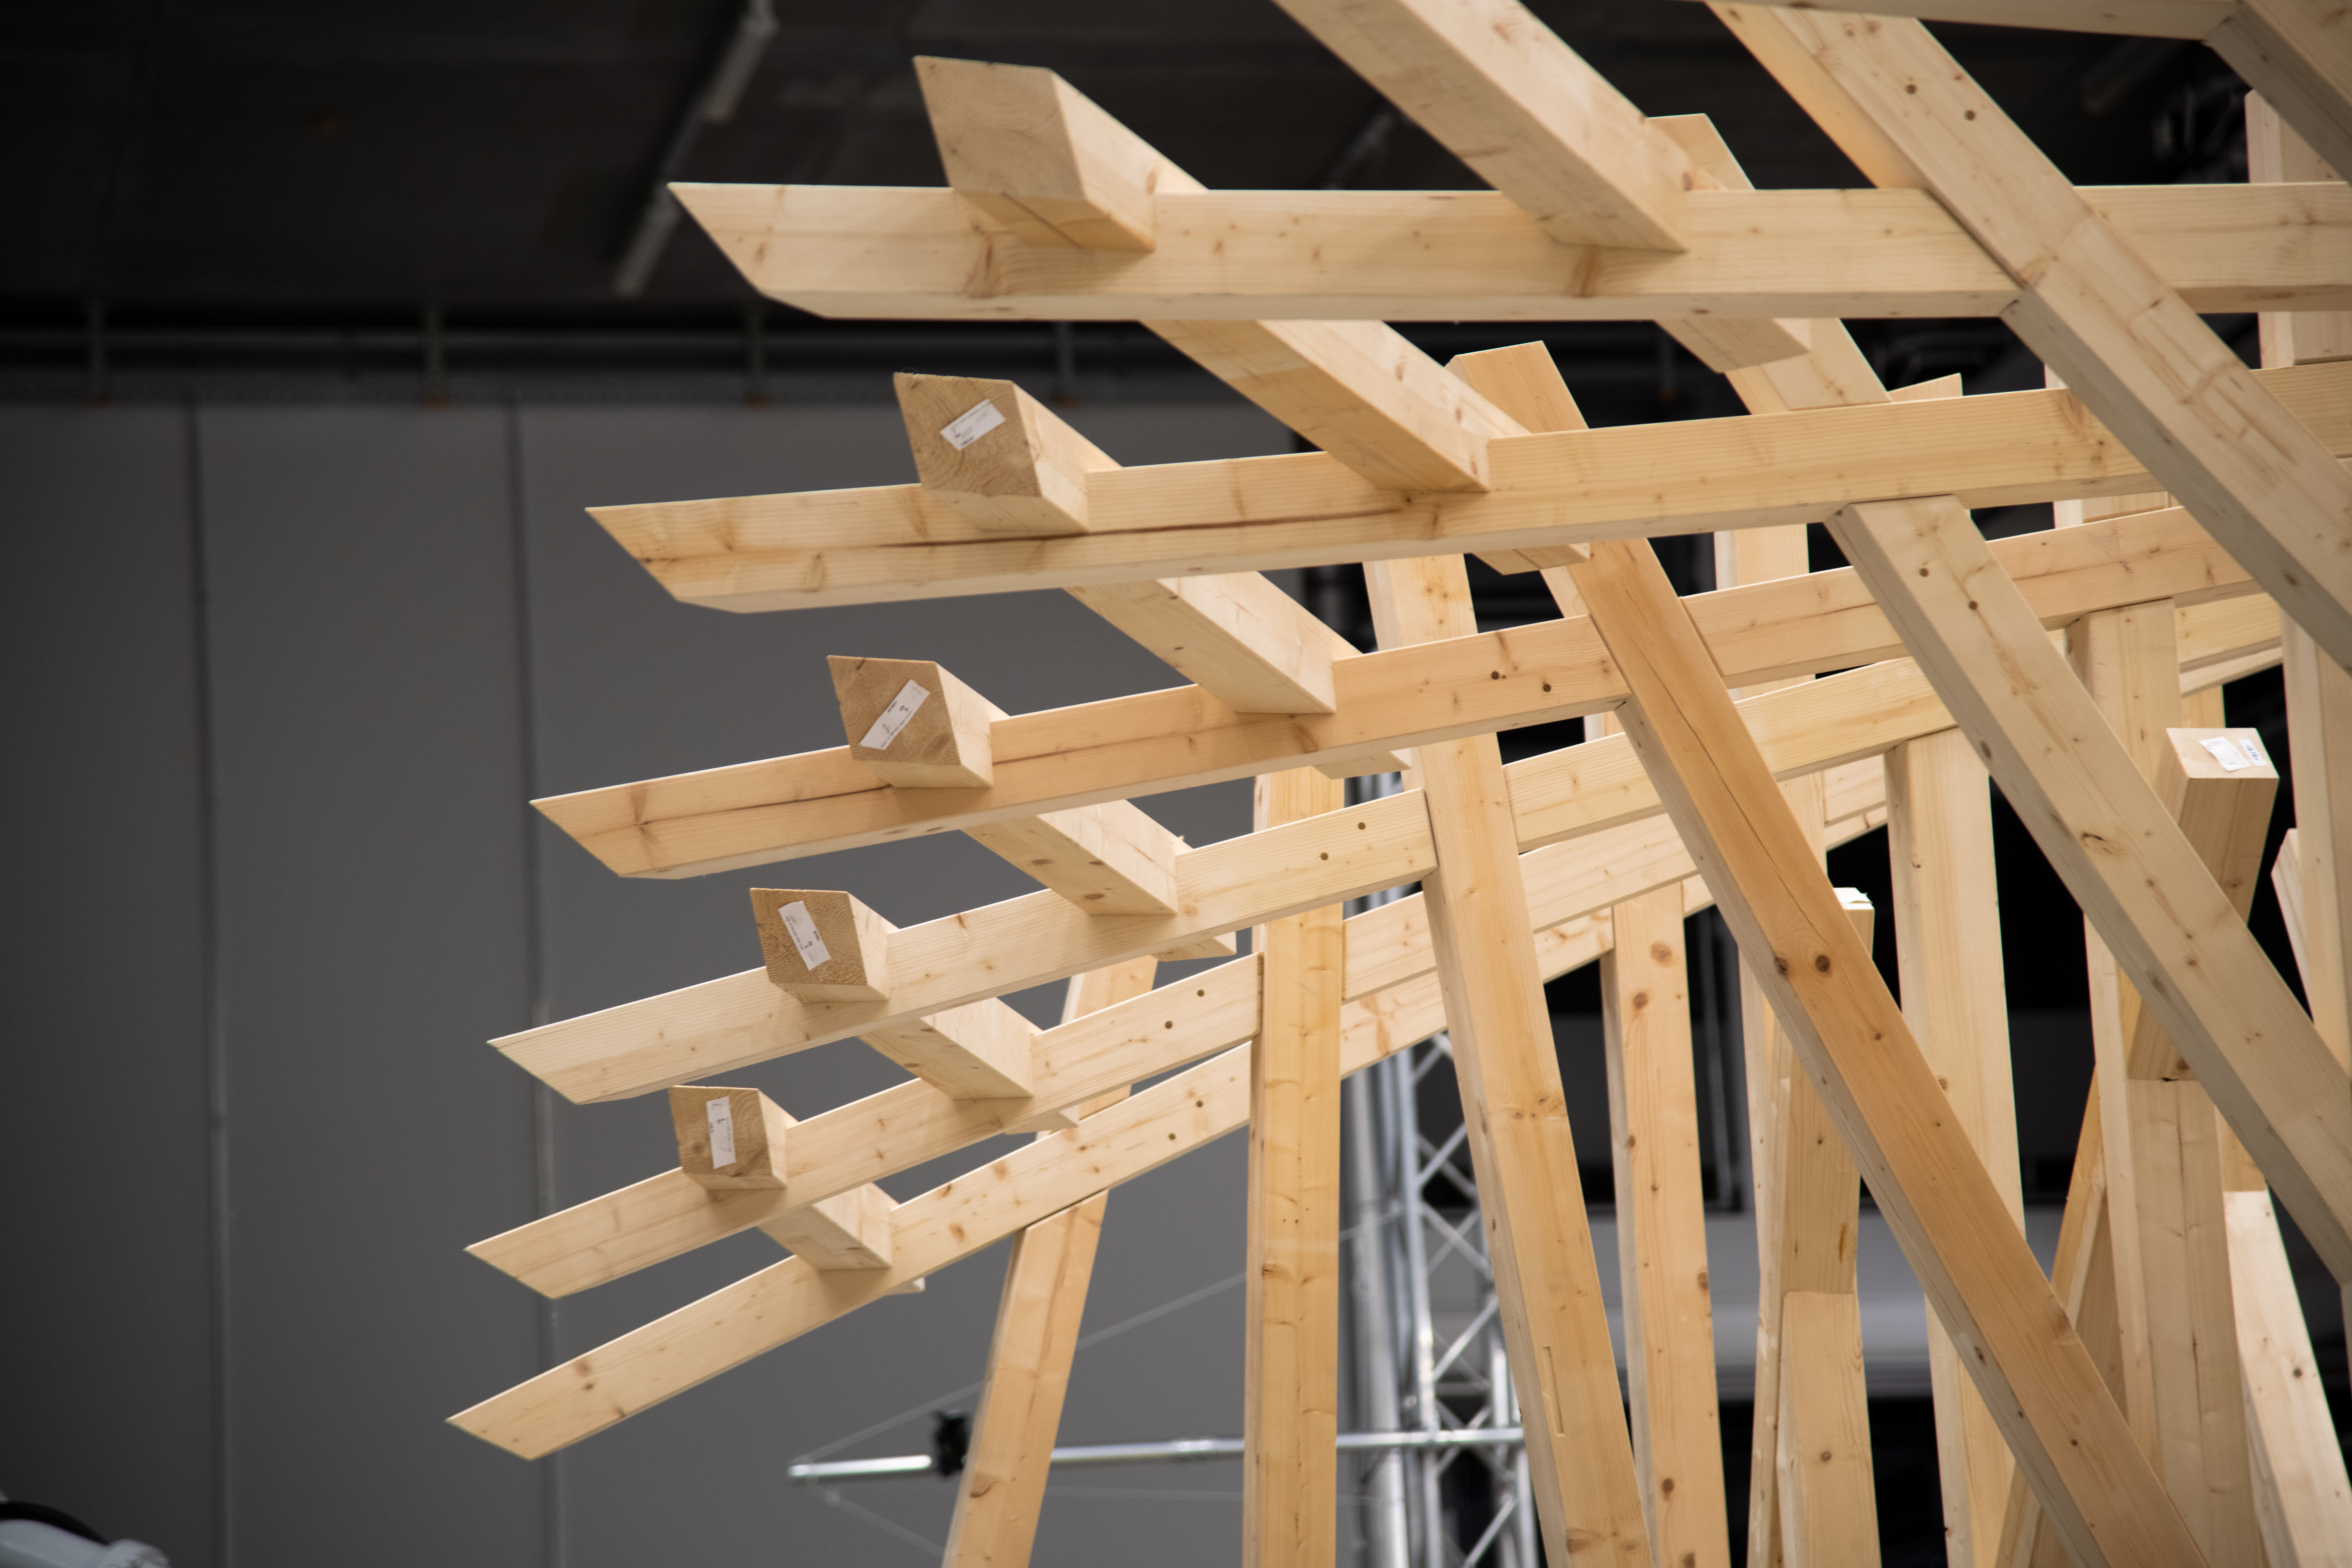
\includegraphics[width=\textwidth]{./images/image6.jpeg}
\end{subfigure}
\hfill
\begin{subfigure}[b]{0.45\textwidth}
\centering
\includegraphics[width=\textwidth]{./images/image7.jpeg}
\end{subfigure}
\end{figure}


The two images below show the cases where the screwdriver SL1 (image below, left) and SL1\_G200 (image below, right) were used to hold the beam. When using the SL1\_G200, the production engineer can choose the orientation of the screwdriver to avoid the long side causing collision with nearby screwdrivers (image below, right). 

\begin{figure}[H]
\centering
\begin{subfigure}[b]{0.45\textwidth}
\centering
\includegraphics[width=\textwidth]{./images/image8.jpeg}
\end{subfigure}
\hfill
\begin{subfigure}[b]{0.45\textwidth}
\centering
\includegraphics[width=\textwidth]{./images/image9.jpeg}
\end{subfigure}
\end{figure}


For a beam that uses multiple screwdrivers, such as the case in the image below, the production engineer can select which screwdriver is the one attached to the robot (deep blue) and the other will be hanging from the beam (deep green).

\begin{figure}[H]
\includegraphics[width=15.92cm,height=7.97cm]{./images/image10.jpeg}
\end{figure}


\vspace{1\baselineskip}
The planned trajectory visualisation interface was also improved with a slider that allows a detailed view of a specific moment to debug potential problems. The image below shows the visualisation halfway during a free motion that transfers a beam. The blue line traces out the vertices of the attached mesh along the motion.

\begin{figure}[H]
\includegraphics[width=15.92cm,height=9.81cm]{./images/image11.jpeg}
\caption{Compute Object States), the serialised Process Model became very large and caused an unpleasant slowdown during serialisation and deserialisation. A new solution was developed to eliminate storing the states explicitly.}
\label{fig:compute_object_states_serialised_process}
\end{figure}


\subsubsection{Action as State Diff Model}

This is achieved by storing only the planned tasks and parsing the tasks dynamically to retrieve the object states at a specific step. This was found to be no different from the already implemented UpdateState() function in each task (diagram below), where the ending state of a task can be computed from the starting state. 

\begin{figure}[H]
\includegraphics[width=11.73cm,height=1.54cm]{./images/image12.jpeg}
\end{figure}


This means that there is a dual relationship between the task and the states. Given an initial state, and the task list, it is possible to derive all the intermediate states and the final state. The following diagrams are the same as before \textit{(see \uline{6.3.5.5 Compute Object States})}. The only difference is that except for the initial state (yellow box), all the other states are not stored (hatched yellow boxes). In practice, the dynamic parsing was found to be much faster than serialisation and deserialisation.

\begin{figure}[H]
\includegraphics[width=8.16cm,height=9.14cm]{./images/image13.jpeg}
\end{figure}


This concept, although simple, is essential for the implementation of automatic Task and Motion Planning (TAMP) in the next Dev Round \textit{(see \uline{8.3.5 Specifying Actions and Goals for TAMP with PDDLStream})}.

\subsubsection{Flowchart for Screwdriver Assembly}

\begin{figure}[H]
\includegraphics[width=15.92cm,height=23.42cm]{./images/image14.jpeg}
\caption{Task Planning with Flowchart) was used for planning the Screw Assembly Process. The diagram below shows the flowchart used for this round. It supports using either a parallel gripper or a screwdriver to hold the beam. The process design and planning workflow is the same as the last round.}
\label{fig:task_planning_flowchart_was_used}
\end{figure}


\subsubsection{Fast Design Validation with IK Check}

The Fast Design Validation by IK was developed to extend the checking function developed in \uline{5.5.2 Checking Incorrect Planning Inputs}. 

In the previous iteration, the check was developed as a developer tool for identifying programming errors before Motion Planning (MP). However, it was found to be useful also during the Process Design Phase for the Production Engineer to detect \textbf{collisions }in the motion request before committing to the slow MP process. Its fast computation speed, requiring only two Collision Check (CC) per Robot Motion Task, was helpful for catching mistakes. For example, all the motions in the BusStop task list can be checked in 1 minute. 

The new extension to the original checking function includes the option to also check for \textbf{reachability}. Reachability refers to whether the robot can reach the defined start and end location for the motion request, taking also into account the collision of the robot body. This is achieved by computing IK for the robot pose at the start and end of the robotic motion. Similar to MP, IK is also stochastic in nature and therefore maximum computation time or maximum retries has to be specified. If the IK solver cannot find a solution within the limits, the motion can be flagged as ‘potentially unreachable’.

This validation check was for the current and next demonstrators. It is used during the transition from the Assembly Design to Process Design Phase to quickly validate the constructability of the design. It provided a better estimation compared to performing CC alone but at a fraction of the time needed for complete MP. The table below shows a comparison of the computation time needed to check the demonstrator for this DevRound \textit{(see \uline{7.4.3 Demonstrator Design  - HyparHut Pavilion})}:

\begin{table}[H]
\begin{adjustbox}{max width=\textwidth}
\begin{tabular}{p{3.36cm}p{3.12cm}p{5.34cm}p{3.94cm}}
\hline
\multicolumn{1}{|p{3.36cm}}{} & 
\multicolumn{1}{|p{3.12cm}}{{\footnotesize \textbf{Collision Check}}} & 
\multicolumn{1}{|p{5.34cm}}{{\footnotesize \textbf{Reachability Check (CC + IK) }}} & 
\multicolumn{1}{|p{3.94cm}|}{{\footnotesize \textbf{Motion Planning}}} \\ 
\hline
\multicolumn{1}{|p{3.36cm}}{{\footnotesize \textbf{Computation Time}}} & 
\multicolumn{1}{|p{3.12cm}}{{\footnotesize < 1 minute}} & 
\multicolumn{1}{|p{5.34cm}}{{\footnotesize < 5 minutes}} & 
\multicolumn{1}{|p{3.94cm}|}{{\footnotesize > 8 hours}} \\ 
\hline
\end{tabular}
\end{adjustbox}
\end{table}
\vspace{2\baselineskip}
\subsubsection{Planning Order by Motion Group}

The non-sequential planning method described in \uline{6.3.7 Non-Sequential Planning Order} was improved and generalised to automatic planning priority. This removed the need for the Process Engineer to manually designate the ‘priority flag’ in the High-Level Task template. 

The idea is to group the tasks in the planned task list into \textbf{Linear Motion Group (LMG)} and \textbf{Free Motion Group (FMG)} and plan them separately. Refer to the diagram below, which depicts a hypothetical task list that consists of LM (green) and FM (blue) while all the non-robotic movements are hidden. The left column shows the groupings, which are simply created by slicing the list wherever LM and FM meet. 

The planning method is to plan each of the LMGs first. If the group does not contain a fixed robot config (M6, M7), sequential planning is used (e.g. M6, M7). If the group contains a fixed config, such as C3 in the first LMG, the motions that are in contact with the fixed config should be planned first (M3, M4) and the planning order is propagated outwards toward the two ends of the group (M2). After all the LMGs are planned, the FMG can be planned using any order. 

\begin{figure}[H]
\includegraphics[width=15.92cm,height=17.04cm]{./images/image15.jpeg}
\end{figure}


The backtracking logic of the algorithm are as follows:

\begin{enumerate}
	\item Planning failures within a LMG should initiate a retry within the group (relying on the stochastic IK behaviour for a different starting configuration). If group retry attempts are exhausted, the LMG is flagged as a failure. 

\begin{enumerate}
	\item If this planning is used for design validation, it is still possible to continue planning other groups. 

	\item If this planning is for execution. The entire planning has failed. The retry threshold can be increased and tried again.

\end{enumerate}
	\item Planning failures within a FMG should initiate a retry within the group (replan all the containing motions). If group retry attempts are exhausted, a larger backtracking step can be pursued:

\begin{enumerate}
	\item The two neighbouring LMGs are replanned and the failed FMG is then retried. If this is successful, replan also the further away FMG neighbours of the replanned LMG because they were invalidated. Using the above diagram as an example, if the FMG (M8) fails, the backtrack will first affect LMG (M6, M7) and LMG (M9, M10). If successful, the FMG (M5) and FMG (M11) will also need to be replaced.

	\item If this multi-group retry attempt allowance is exhausted, the failure procedure can be similar to that of LMG in step 1a and 1b.

\end{enumerate}
\end{enumerate}
This non-sequential planning order was tested extensively during the Process Design Phase of the HyparHut and CantiBox. The following benefits have been observed:

\begin{itemize}
	\item The constraining robot configuration is automatically propagated, removing the need for manually assigning a planning order, which could be prone to error.

	\item The LMGs are always independent from each other and can be planned separately, or computed in parallel using different computers.

	\item Fine-grained back tracking (compared to retrying all motions for a beam)

\begin{itemize}
	\item Improved planning efficiency

	\item The failure of a specific LMG provides a good indication of where the problems are.

\end{itemize}
	\item LMG typically only contains a few LMs, they can also be planned very fast because no FM are involved. This is potentially useful for real-time design checking for a small group of actions (this use is not tested).

\end{itemize}
During the Process Design phase of the two demonstrators, LMG planning (without proceeding to FMG) was used as a more detailed check than the CC+IK method\textit{ (see \uline{7.3.21 Fast Design Validation with IK Check)}}. The computing time is roughly 10 to 15 minutes (depending on how many failures) for the HyparHut Pavilion. This duration is found to be acceptable as a final check before the rest of the FMG is planned, which requires significantly longer time ($\sim$ 8 hours).

\subsubsection{Post-Planning Trajectory Smoothing}

In order to address the problem related to low-quality motion planning results from RRT-Connect. Trajectory smoothing using Random Shortcut \href{https://www.zotero.org/google-docs/?kdUrGV}{(Zhao $\&$ Sidobre, 2015)}\textit{ }was implemented in the planning workflow for reducing the robot travel distance and time.

The image below shows an example of the robot travelling with the PG1000 gripper towards the beam pickup location. The difference between the two trajectories can be seen before (top) and after trajectory smoothing (bottom). 

\begin{figure}[H]
\centering
\begin{subfigure}[b]{0.45\textwidth}
\centering
\includegraphics[width=\textwidth]{./images/image16.jpeg}
\end{subfigure}
\hfill
\begin{subfigure}[b]{0.45\textwidth}
\centering
\includegraphics[width=\textwidth]{./images/image17.jpeg}
\end{subfigure}
\end{figure}


\subsection{Demonstration}

\subsubsection{Design Goal}

There are many goals for the design of the demonstrator in this round:

\section{Process Validation}

\begin{itemize}
	\item \textbf{Validate stability awareness} (based on my intuition while stepping through each step) to avoid using scaffolding \textit{(see \uline{7.1.1 Deformation-Awareness and Error Correction by Triangulation})}.

	\item \textbf{Validate operation of SL1 Screwdriver - }\textit{(see \uline{7.3.7 Lap Screwdriver SL1 and SL1\_G200 Hardware})}

	\item \textbf{Validate operation of SL1\_G200 Screwdriver as a gripper}

	\item \textbf{Validate the assembly of}

\begin{itemize}
	\item \textbf{Polyline lap joints} - Customised with traditional lap joints details \textit{(see \uline{7.3.1 Parametric Polyline Lap Joints})}

	\item \textbf{Non-planar lap joints }- Only possible with the Screw Assembly Method \textit{(see \uline{7.3.2 Parametric Non-Planar Lap Joints})}

	\item \textbf{Elements with different sizes} - First attempt of different beam sizes according to structural requirements. 

\end{itemize}
	\item \textbf{Validate anchoring horizontal elements} - instead of anchoring vertical elements in the previous attempts, to improve initial stability.

\end{itemize}
\section{Architectural Design Demo}

\begin{itemize}
	\item \textbf{Demonstrate a Hut Typology} - Post and column framing walls, supporting a roof).

	\item \textbf{Contains framing structures} - Demonstrate framing of walls, floors using primary and secondary elements.

	\item \textbf{Hyperbolic Paraboloid Roof Surface} - Demonstrate structural complexity that is achievable with non-planar joints. 

\end{itemize}
\subsubsection{Design and Team Information}

MISSING TABLE

\vspace{1\baselineskip}
\subsubsection{Demonstrator Design - HyparHut Pavilion}

The designed structure is a column grid framing with a hyperbolic roof. The typology is similar to a hut. The grid consists of 2 rows of 3 columns. However, one of the columns is stopped short and does not touch the roof. This creates a cantilevered corner for the curved roof.

\uline{\begin{figure}[H]
\includegraphics[width=15.92cm,height=8.96cm]{./images/image18.jpeg}
\end{figure}
}

The roof consists of two primary beams that are supported by the columns. The size of the primary beams was 100mm x 140mm to simulate the need for more structural depth, but also to test the assembly of larger and heavier (>30kg) elements.

The primary beams supported a set of seven secondary beams that are arranged in an orthogonal direction. These beams are 100mm x 120mm. The lap joints between these two sets of beams are interlocking with parallel surfaces to provide mutual stability. 

\begin{figure}[H]
\includegraphics[width=14.33cm,height=8.67cm]{./images/image19.jpeg}
\end{figure}


A top layer of smaller roof elements, with a size of 100mm x 100mm, is added to create a more defining roof surface. The Elements are split into discontinued members to avoid having too many simultaneously assembled joints (there are only 4 screwdrivers available) and allow the axial rotation of the elements to follow the curvature of the hyperbolic paraboloid surface. 

The top layer elements are split into a pattern of 2 + 4 + 2 spans and 3 + 2 + 3 spans. This maximises the structural continuity of the surface when compared to splitting all elements at the same location. It also produces a visually pleasing pattern. Moreover, this allows the testing of the assembly process with elements that have 2, 3, and 4 simultaneous joints. The image below shows the assembly scenario for 2 simultaneous joints (image below, left) and for 4 simultaneous joints (image below, right).

\begin{figure}[H]
\centering
\begin{subfigure}[b]{0.45\textwidth}
\centering
\includegraphics[width=\textwidth]{./images/image20.jpeg}
\end{subfigure}
\hfill
\begin{subfigure}[b]{0.45\textwidth}
\centering
\includegraphics[width=\textwidth]{./images/image21.jpeg}
\end{subfigure}
\end{figure}


The photo below shows the top layer elements. Notice that the beams are rotated to follow the local curvature of the surface. An edge chamfer was added at the intersection of these beams to smooth out the abrupt visual change between the axial rotation.

\uline{\begin{figure}[H]
\includegraphics[width=15.92cm,height=10.62cm]{./images/image22.jpeg}
\end{figure}
}

A manually-assembled floor system was included to simulate an architectural programme and to provide some utility purpose after the structure is built. It has two levels, each with a different spanning direction. A dovetailed joint was used for these beams (photo below, left), which were not assemblable by the clamps or the screwdrivers, this was intentionally included to understand the joint better. The floor plates were CLT plates that are simply supported in a recessed groove on the floor beams.

\begin{figure}[H]
\centering
\begin{subfigure}[b]{0.45\textwidth}
\centering
\includegraphics[width=\textwidth]{./images/image23.jpeg}
\end{subfigure}
\hfill
\begin{subfigure}[b]{0.45\textwidth}
\centering
\includegraphics[width=\textwidth]{./images/image24.jpeg}
\end{subfigure}
\end{figure}


The design of the joints using the polyline lap customization allows sophisticated joint details that were customised according to structural requirement. For example, a dovetail profile was used for the diagonal joints that need to withstand tension. Various shoulder details were used to improve load bearing capacity for a specific loading direction.

\uline{\begin{figure}[H]
\centering
\begin{subfigure}[b]{0.23\textwidth}
\centering
\includegraphics[width=\textwidth]{./images/image25.jpeg}
\end{subfigure}
\hfill
\begin{subfigure}[b]{0.23\textwidth}
\centering
\includegraphics[width=\textwidth]{./images/image26.jpeg}
\end{subfigure}
\hfill
\begin{subfigure}[b]{0.23\textwidth}
\centering
\includegraphics[width=\textwidth]{./images/image27.jpeg}
\end{subfigure}
\hfill
\begin{subfigure}[b]{0.23\textwidth}
\centering
\includegraphics[width=\textwidth]{./images/image28.jpeg}
\end{subfigure}
\end{figure}
}

\subsection{Lessons Learnt}

\subsubsection{Execution Plan}

Similar to the BusStop demonstrator, the preparation procedures were similar. However, unexpected discovery of CNC error in the prefabricated added some complexity to the preparation. The preparation consisted of the following tasks:

\begin{enumerate}
	\item Export beam geometry to Cadwork and sent to Fabricator for machining

	\item Construct and calibrate aluminium foundation 

	\item Replan motions with updated collision models and taught configurations

	\item Inspect the received CNC machined beams

\begin{enumerate}
	\item Test fit planar frame on the ground

	\item Adjust inaccurate joints  \textit{(see \uline{7.5.3 Missing Cut Problem})}

\end{enumerate}
	\item Adjust inaccurate machined-holes \textit{(see \uline{7.5.4 Inaccurate Screw Hole Problem})}

\begin{enumerate}
	\item Test fit entire pavilion\textit{ (see notes below)}

	\item Redrill misaligned holes

	\item Chamfer screw hole entry

	\item Drill pin gripper attachment holes \textit{(similar procedure to \uline{7.5.1.1 Pin Gripper Holes Drilling Jig})}

\end{enumerate}
	\item Chamfer joint edges \textit{(similar to the method used in \uline{5.6.6 Clamping Joints with Chamfered Edges}, except 4mm was used)}

	\item Robotic Assembly\textit{ (refer to \uline{7.3.20 Flowchart for Screwdriver Assembly})}

\begin{enumerate}
	\item Robot picks up a parallel gripper or uses a screwdriver as a gripper.

	\item Operator load material.

\begin{enumerate}
	\item Operator places a beam in the gripper.

	\item Operator places hollow screws on screwdrivers.

	\item Operator attaches screwdrivers to the beam.

\end{enumerate}
	\item The robot transfers the beam and screwdrivers to the PA structure.

	\item The robot and screwdrivers move synchronously to tighten the joint.

	\item The robot retrieves the used screwdriver one by one, returning them to storage.

\end{enumerate}
\end{enumerate}
The preparation period for this demonstrator was long because of the various manual drilling operations (planned and expected) and adjustment of inaccurate CNC machined features (unexpected). Moreover, the hole misalignment problem required a complete test fit of the whole pavilion for diagnosing and correction. In total, the diagnosis and adjustment process took almost 10 days. \textit{(see }7.5. \cite{no_auth_4}.1 Correction of the Screw Holes\textit{)}

 The photo below (left) shows the timber beams received from the fabricator before any adjustments. The photo on the right shows the CLT plates for the manually-assembled floor.

\begin{figure}[H]
\centering
\begin{subfigure}[b]{0.45\textwidth}
\centering
\includegraphics[width=\textwidth]{./images/image29.jpeg}
\end{subfigure}
\hfill
\begin{subfigure}[b]{0.45\textwidth}
\centering
\includegraphics[width=\textwidth]{./images/image30.jpeg}
\end{subfigure}
\end{figure}


After the inaccurate joints and drill holes were corrected. The assembly area was prepared. The photo below shows the construction area and the various features. The operator’s console is established as a fixed location at the edge of the construction area to simulate an industrial setting.

\begin{figure}[H]
\includegraphics[width=15.92cm,height=8.96cm]{./images/image31.png}
\end{figure}


The location of all the fixed objects are measured by the iGPS system and modelled in the CAD environment. This is used to update the collision geometry that was modelled by estimation during the validation stage. The image below shows the updated collision geometry (orange) covering all the fixed objects in the construction area. 

\begin{figure}[H]
\includegraphics[width=15.92cm,height=7.97cm]{./images/image32.jpeg}
\end{figure}


The photos below show the four screwdrivers (left) and the three parallel grippers (right) in their storage location. Taught configurations of these positions were acquired using the robot for replanning the motions. 

\begin{figure}[H]
\centering
\begin{subfigure}[b]{0.45\textwidth}
\centering
\includegraphics[width=\textwidth]{./images/image33.jpeg}
\end{subfigure}
\hfill
 \begin{subfigure}[b]{0.45\textwidth}
\centering
\includegraphics[width=\textwidth]{./images/image34.jpeg}
\end{subfigure}
\end{figure}


The images below show the collision models (CM) used for the screwdriver storage area. The plastic storage pads (left image, blue under orange) can be seen covered by a static box-shape CM (orange) to protect them. When the tools are placed in the storage location (right image), the CM of the tools (from the Tool Model) will protect itself.

Note that the CM of the storage pad is in collision with the tool at the stored location (right image). This is only possible because the ACM of the planning call is programmed to ignore these collisions \textit{(refer to \uline{5.2.7.1 Collision Checking})}. This is set in the High-Level Task templates \textit{(refer to }6. \cite{no_auth_3}.5.2 Expansion to Low Level Tasks\textit{)} for the Linear Motions going to and from the storage location.

\begin{figure}[H]
\centering
\begin{subfigure}[b]{0.45\textwidth}
\centering
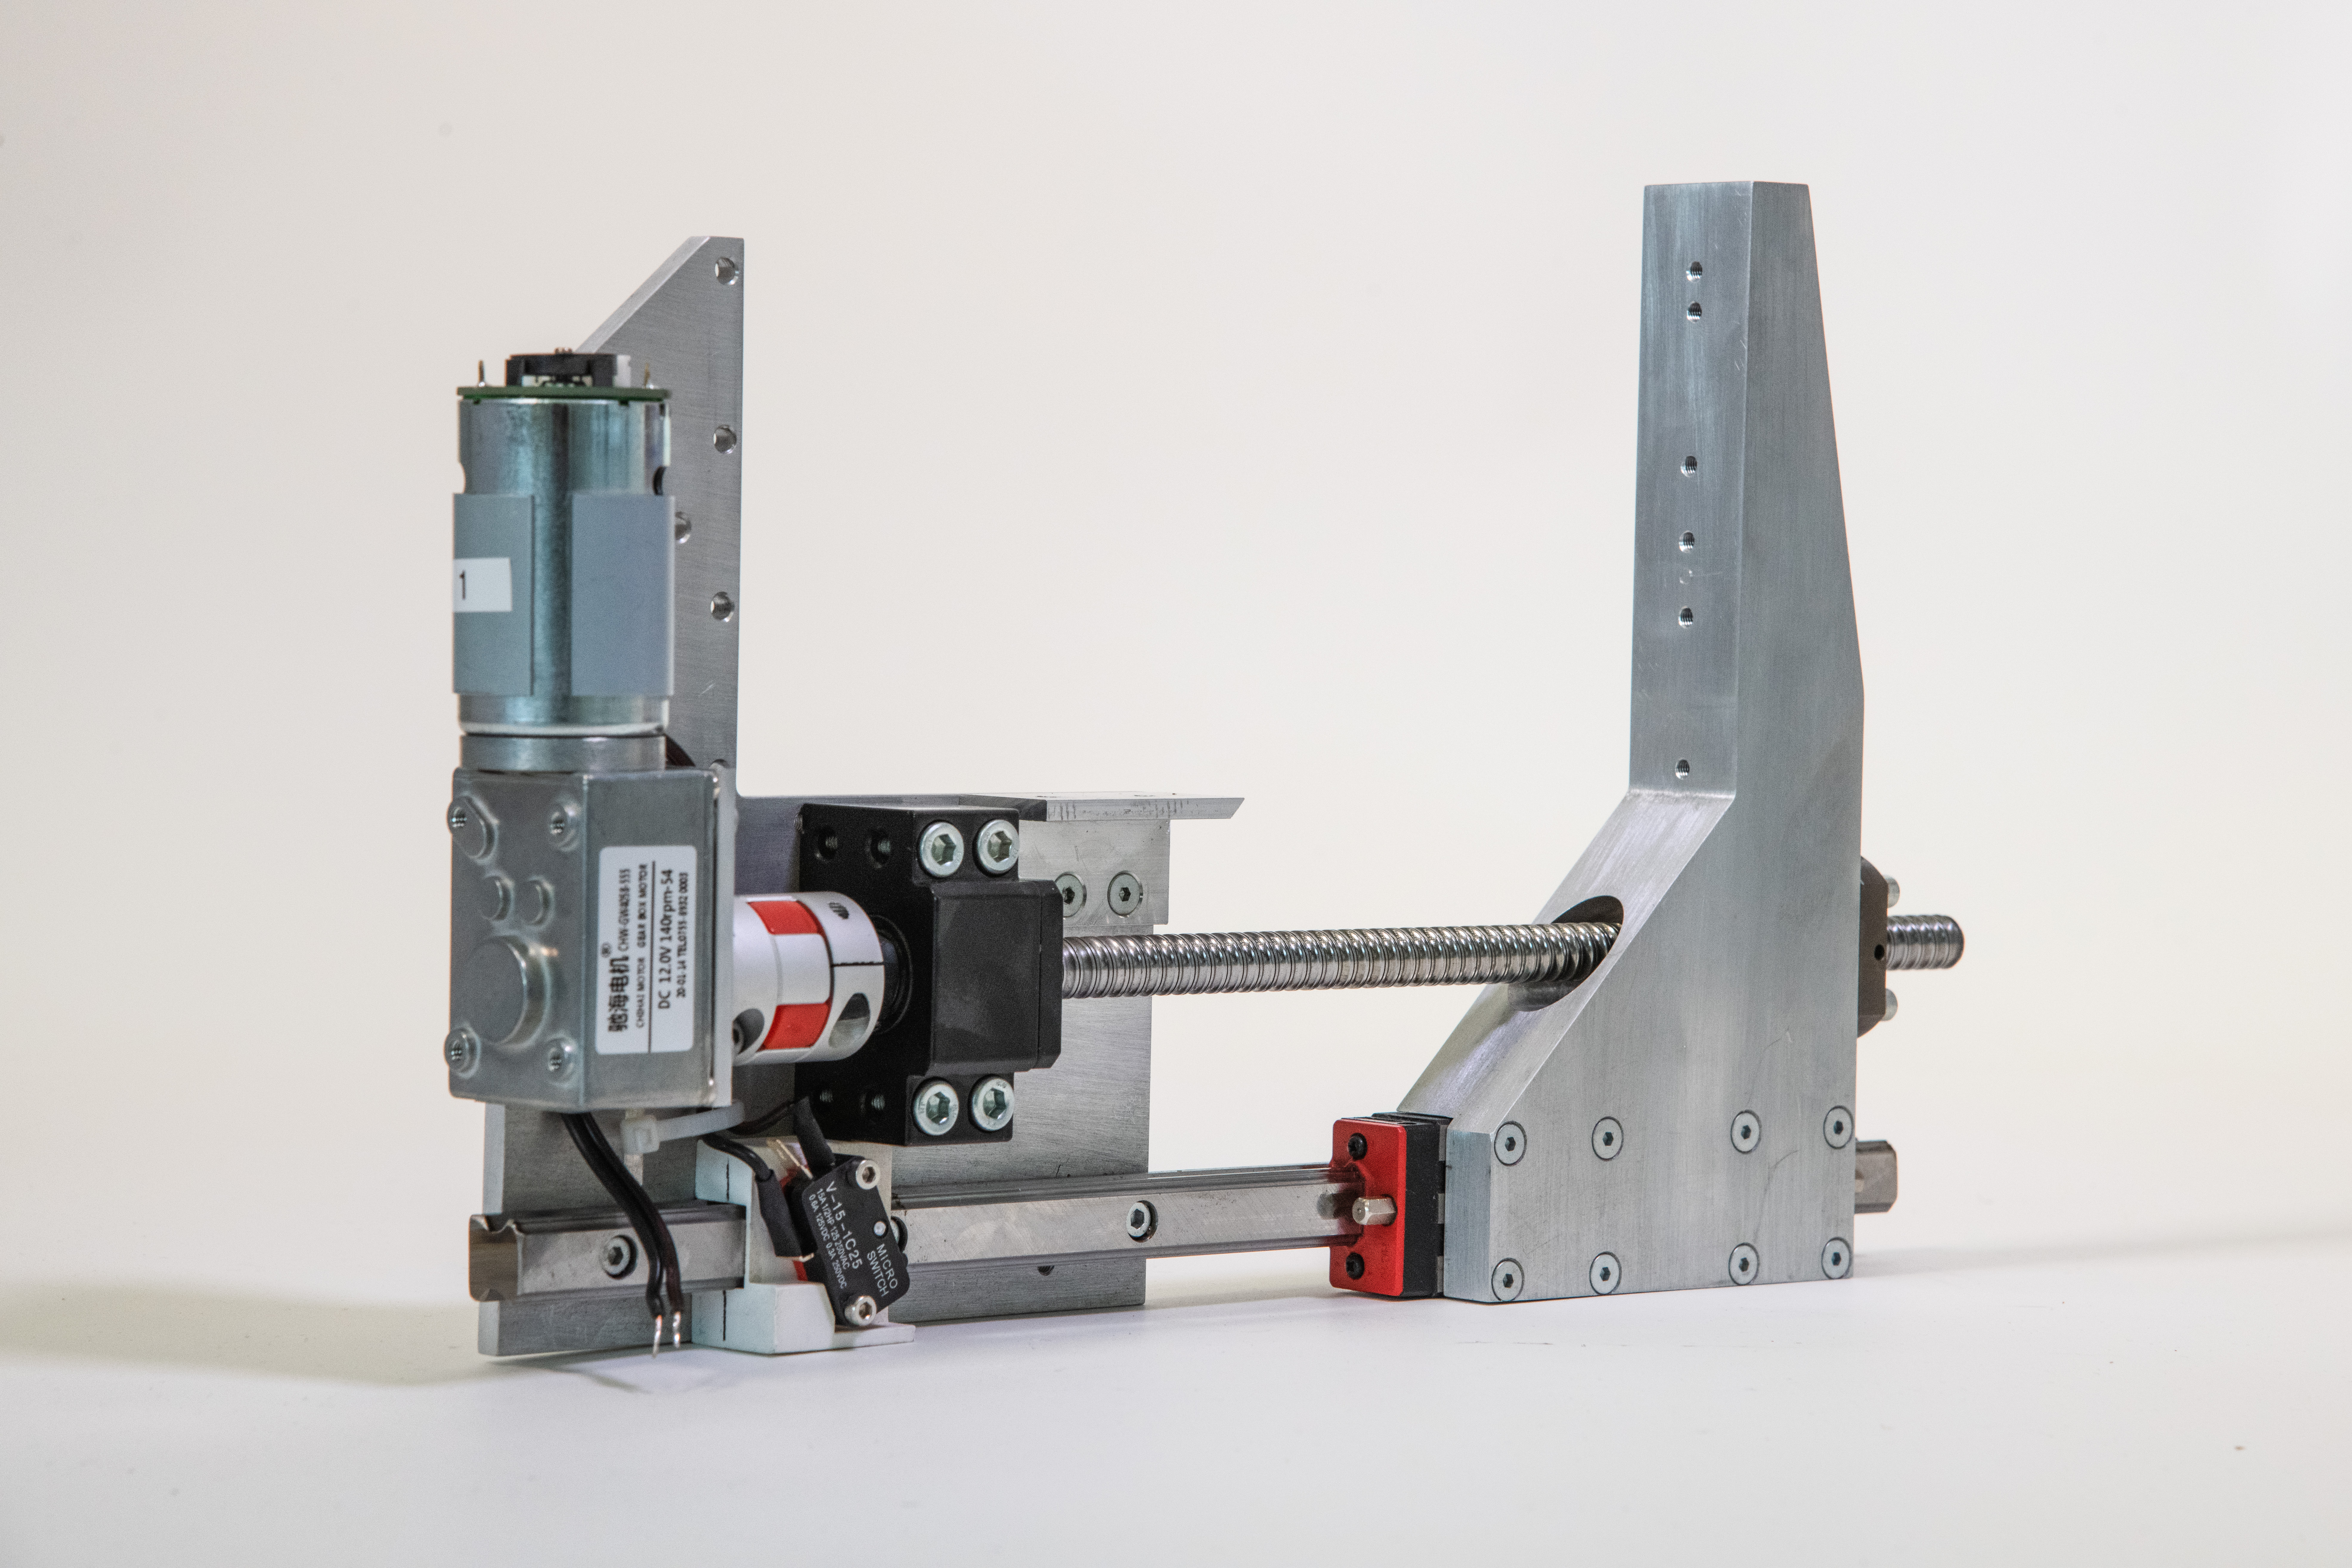
\includegraphics[width=\textwidth]{./images/image35.jpeg}
\end{subfigure}
\hfill
\begin{subfigure}[b]{0.45\textwidth}
\centering
\includegraphics[width=\textwidth]{./images/image36.jpeg}
\end{subfigure}
\end{figure}


The photo below shows the screws prepared for the construction. The short screws (lower left box) are used for all the planar lap joints. The long screws (other boxes) are used for all the non-planar lap joints.

\begin{figure}[H]
\includegraphics[width=15.92cm,height=8.96cm]{./images/image37.jpeg}
\end{figure}


\subsubsection{Successful Validation}

The pavilion was successfully constructed with a high degree of automation \textit{(see \uline{7.5.2.12 Automated Process})}. It validated many new developments in this Dev Round and showed progressive improvement in reducing manual interventions required during the robotic process. This section will elaborate on these successful validations, while later sections will describe the more problematic issues.

The photo below shows the completed pavilion, including the manually assembled floor.

\begin{figure}[H]
\includegraphics[width=15.92cm,height=8.96cm]{./images/image18.jpeg}
\end{figure}


\paragraph{Screwdriver Joint Closure}

This demonstration was the first time the SL1 and SL1\_G200 Screwdriver were tested with a robot. The following functions have been validated:

\section{Joint Closure and Left-In Screw}

The main function of the screwdriver to close lap joints performed as designed. The design of the pull screw, selection of gearbox and main motor all performed as expected. As long as the pull screw tip entered the hole on the stationary-side during initial contact, the screwdriver was able to successfully close the joint. 

Screwed operations were used for 54 out of 57 beams (except the first three beams connected to the platform). A total of 125 joints were screwed without problems. There were no motor stalling observed.

The photos below show a \textbf{typical operation sequence} of the closure:

\begin{enumerate}
	\item Screwdriver and beam tip arrives at the approach position. The synchronous motion of the robot (linear motion) and the screwdriver (rotation) begins. The receiving hole has a chamfer for providing passive correction.

	\item The chamfered edges on the joint engage, guiding the alignment until parallel surfaces of the lap joint engage. The hollow screw will engage with the stationary-side.

	\item The lap joint is closed. The screwdriver switches to torque control mode to further tighten the hollow screw to a calibrated torque.

	\item The screwdriver is retracted with another synchronous motion with the robot. Different from step 1, the pull screw rotates counterclockwise while the robot moves backwards. The hollow screw is left in the joint.

\end{enumerate}
1\includegraphics[width=7.16cm,height=4.03cm]{./images/image38.jpeg} 2\includegraphics[width=7.16cm,height=4.03cm]{./images/image39.jpeg} \\ 3\includegraphics[width=7.16cm,height=4.03cm]{./images/image40.jpeg} 4\includegraphics[width=7.16cm,height=4.03cm]{./images/image41.jpeg}

\paragraph{Screwdriver as a Gripper}

The screwing assembly process supported two different gripping modes. Both of them performed as intended. Refer to the two photos below:

\begin{enumerate}
	\item A parallel gripper is used by the robot to hold the beam. Other screwdrivers are attached to the beam and move with it. (Tested on 23 beams)

	\item The robot directly holds a screwdriver and the beam is attached to the screwdriver by the pin grippers of the screwdriver.  (Tested on 34 beams)

\end{enumerate}
{\small 1\includegraphics[width=7.64cm,height=4.3cm]{./images/image42.jpeg}2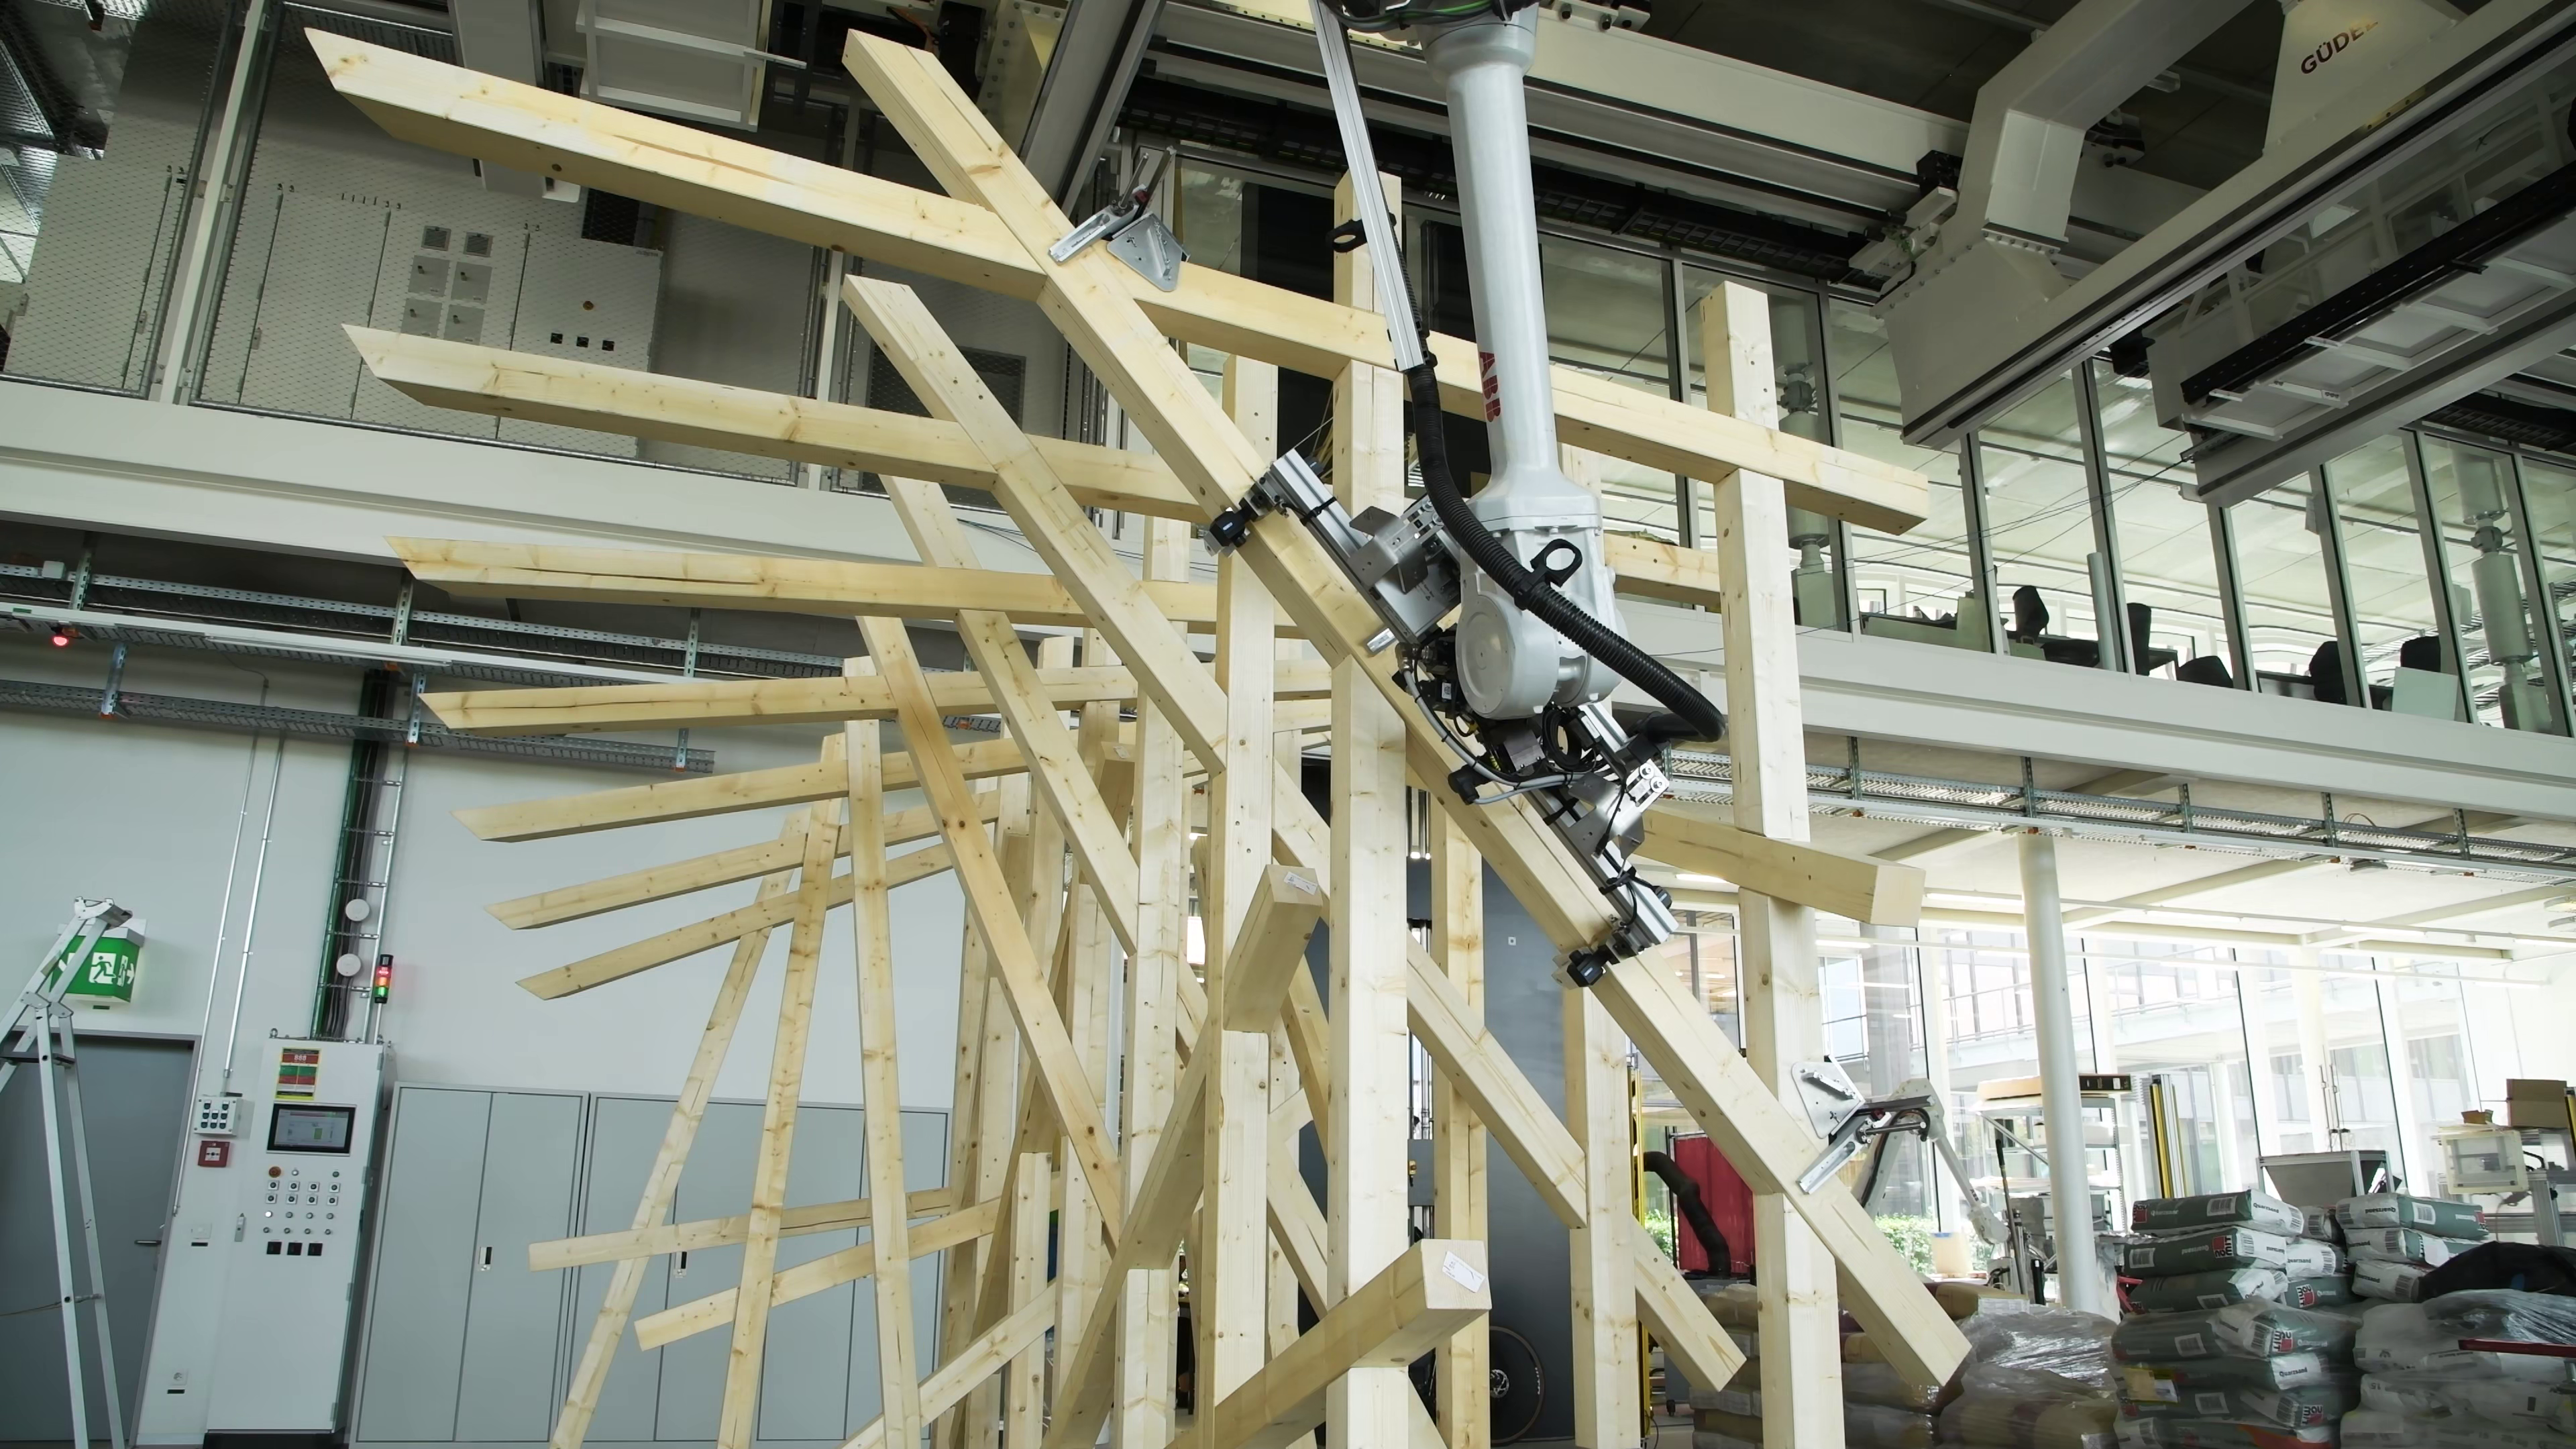
\includegraphics[width=7.64cm,height=4.3cm]{./images/image43.png}}

The screwdriver-as-gripper method was tested with SL1 and SL1\_G200 Screwdriver. The image below shows the SL1\_G200 holding a 3.1m long beam while three other screwdrivers are attached to the beam. This validated the strength of the pin gripper mechanism.

\begin{figure}[H]
\includegraphics[width=15.92cm,height=8.96cm]{./images/image44.png}
\end{figure}


The following gripper selection guide summarised the lesson learnt during the design process and the observation from the demonstration:

\begin{itemize}
	\item In general, always use a parallel gripper if its size does not cause a collision problem. Choose the biggest gripper size possible for the beam length.

	\item If parallel gripper cannot be used, use the longer SL1\_G200 if possible. Pick a joint near the middle of the beam length to avoid imbalance deflection.

	\item If collision is still a problem, SL1 can be used. However, it is not recommended for long elements.

\end{itemize}
The following images show the imbalance grasp caused by using the screwdriver as a gripper. In this case, the spacing between the four joints does not permit the use of any parallel grippers. The even number of joints on the beam also means that it is not possible to hold it near the centre using the screwdriver as a gripper method. This type of scenarios occurred 5 times during construction and they often suffer from misalignment problems \textit{(see \uline{7.5.6 Screwdriver Tip Misalignment})}

\begin{figure}[H]
\centering
\begin{subfigure}[b]{0.45\textwidth}
\centering
\includegraphics[width=\textwidth]{./images/image45.jpeg}
\end{subfigure}
\hfill
\begin{subfigure}[b]{0.45\textwidth}
\centering
\includegraphics[width=\textwidth]{./images/image46.jpeg}
\end{subfigure}
\end{figure}


\paragraph{Fastener Kept Joints From Loosening}

The hollow screws performed their intended role to keep the structure stable during construction. None of the joints have been found to be loosened after they are assembled. This successfully addressed the loosening problem observed in clamped joints \textit{(see \uline{5.6.15 Joints Loosening after Assembly})} and contributed to the overall stability during construction. The photos below show the hollow screw being revealed during (left) and after (right) the screwdriver is retracted with the robot.

\begin{figure}[H]
\centering
\begin{subfigure}[b]{0.45\textwidth}
\centering
\includegraphics[width=\textwidth]{./images/image47.jpeg}
\end{subfigure}
\hfill
\begin{subfigure}[b]{0.45\textwidth}
\centering
\includegraphics[width=\textwidth]{./images/image48.jpeg}
\end{subfigure}
\end{figure}


\paragraph{Loading Beam and Screwdriver}

The operator tasks for loading the beam and the screwdrivers can be observed in the photos below. 

\begin{enumerate}
	\item Robot brings a gripper to the attachment area, aligned to a horizontal surface.

	\item Operator pushes the beam into the gripper, aligning it with the gripper registration features. The horizontal surface can reduce the operator effort.

	\item Robot closes the gripper and brings it upwards.

	\item Robot rotates the beam to the direction where the subsequent grippers can be attached in a downwards orientation.

	\item Operator attach screwdriver

\begin{enumerate}
	\item Operator loads a hollow screw to the screwdriver. The correct screw length must be selected according to design.

	\item Operator inserts the pull screw tip through the hole pre-drilled at the joints. There are two orientations possible, only one is correct.

\end{enumerate}
	\item Operator can use the manual switch to control the tightening and loosening of the pin gripper. 

	\item Operator continues to attach as many screwdrivers as needed.

	\item Robot continues with the automatic process and brings the beam towards the assembly location.

\end{enumerate}
{\small 1\includegraphics[width=7.64cm,height=4.3cm]{./images/image49.jpeg}2\includegraphics[width=7.64cm,height=4.3cm]{./images/image50.jpeg} \\ 3\includegraphics[width=7.64cm,height=4.3cm]{./images/image51.jpeg}4\includegraphics[width=7.64cm,height=4.3cm]{./images/image52.jpeg} \\ 5\includegraphics[width=7.64cm,height=4.3cm]{./images/image53.jpeg}6\includegraphics[width=7.64cm,height=4.3cm]{./images/image54.png} \\ 7\includegraphics[width=7.64cm,height=4.3cm]{./images/image55.jpeg}8\includegraphics[width=7.64cm,height=4.3cm]{./images/image56.jpeg}}

\textbf{Lessons learnt }from the construction experience:

\begin{itemize}
	\item Step 5a is prone to operator error of selecting the wrong screw, an indication would be beneficial for the future.

	\item Step 5b is prone to operator error of using the wrong orientation (occurred two times), a geometrical registration feature can be used to prevent this in the future.

	\item Step 6 is prone to the operator over-tightening the pins and causing jamming after the assembly \textit{(see \uline{7.5.8 Pin Gripper Jammed in Locked State})}. The screwdriver firmware can be improved in the future to provide indication and to stop the pin motion automatically when the correct torque is reached.

\end{itemize}
Alternatively, the hollow screw and screwdriver attachment tasks can be automated. A small robot with 10 kg payload would be sufficient for this task.

\paragraph{Visual-guided Docking Process}

The camera-marker alignment system developed for aligning the docking adapters performed as intended. The photo belows shows the moment during alignment (left) and the moment after the linear movement docks the two halves. 

\begin{figure}[H]
\centering
\begin{subfigure}[b]{0.45\textwidth}
\centering
\includegraphics[width=\textwidth]{./images/image57.jpeg}
\end{subfigure}
\hfill
\begin{subfigure}[b]{0.45\textwidth}
\centering
\includegraphics[width=\textwidth]{./images/image58.jpeg}
\end{subfigure}
\end{figure}


The alignment system was used 125 times for all the PickScrewdriverFromStructure tasks. Except for the times when other problems prevented the screwdrivers to be picked up automatically, all the other alignments were successful.

The table below shows the number of correction attempts before the measured error converged to within tolerance. The convergence threshold is 1.0mm on the XY plane and 0.5mm on the Z direction of the docking adapter flange. Notice that only two attempts were needed in the worst case.

\begin{table}[H]
\begin{adjustbox}{max width=\textwidth}
\begin{tabular}{p{8.61cm}p{7.27cm}}
\hline
\multicolumn{1}{|p{8.61cm}}{{\footnotesize \textbf{Number of Corrections To Converge}}} & 
\multicolumn{1}{|p{7.27cm}|}{{\footnotesize \textbf{Count}}} \\ 
\hline
\multicolumn{1}{|p{8.61cm}}{{\footnotesize \textbf{0 $\ast$}}} & 
\multicolumn{1}{|p{7.27cm}|}{{\footnotesize 3}} \\ 
\hline
\multicolumn{1}{|p{8.61cm}}{{\footnotesize \textbf{1}}} & 
\multicolumn{1}{|p{7.27cm}|}{{\footnotesize 70}} \\ 
\hline
\multicolumn{1}{|p{8.61cm}}{{\footnotesize \textbf{2}}} & 
\multicolumn{1}{|p{7.27cm}|}{{\footnotesize 18}} \\ 
\hline
\end{tabular}
\end{adjustbox}
\end{table}
{\footnotesize $\ast$ No correction needed after marker is detected}

The graph below (left) shows the amount of offset applied as a result of the correction for each attempt. It is representative of the deviation between the constructed structure and the CAD model. The graph below (right) shows the distribution of deviation.

\begin{figure}[H]
\centering
\begin{subfigure}[b]{0.45\textwidth}
\centering
\includegraphics[width=\textwidth]{./images/image59.png}
\end{subfigure}
\hfill
\begin{subfigure}[b]{0.45\textwidth}
\centering
\includegraphics[width=\textwidth]{./images/image60.png}
\end{subfigure}
\end{figure}


{\footnotesize Number of measured data points $=$ 91 \\ Mean Value (after discarding top and bottom 5$\%$ outlier) $=$ 7.5}

The camera-marker alignment system provided not only the active guidance, but also validation of successful alignment. This confirmation prevented the subsequent linear robotic motion from crashing into the tool changer in case of poor alignment. Future followup could consider continuous visual guidance or validation during the linear motion to improve reliability.

The combination of the camera-marker alignment system and the newly added docking lock sensor eliminated the need for the operator to perform a visual check. The two functions performed very reliably when combined and would only notify the operator if the locking action failed. The only minor problem was that the WiFi signal for the wireless video feed was not always reliable and would occasionally drop. In most cases, the connection would be reestablished after randomly adjusting the WiFi access point antennas. 

\paragraph{Global Correction Approach}

The deformation-aware design practice was used in different areas of the structure. The principle relies on identifying high-risk elements that can suffer from deformation (performed by intuition in this demo) and apply strategies that can mitigate the risk:

\begin{itemize}
	\item Change the design or assembly sequence of the unstable element.

	\item Add or modify subsequent elements to form triangles to correct the deviation.

\end{itemize}
The photo below (left) shows the moment after the tallest column is installed. This column was considered to be at high risk of deformation because of its length and because only one joint was connected. The photo on its right shows the horizontal beam that was assembled next. Note that the three mating joints are very close to the other joints below them. With such a short distance to the last accurate point, the deviation for these three joints are also minimal. 

\begin{figure}[H]
\centering
\begin{subfigure}[b]{0.45\textwidth}
\centering
\includegraphics[width=\textwidth]{./images/image61.jpeg}
\end{subfigure}
\hfill
\begin{subfigure}[b]{0.45\textwidth}
\centering
\includegraphics[width=\textwidth]{./images/image62.jpeg}
\end{subfigure}
\end{figure}


In other words, even if the tall column is deformed (in the left photo above), the alignment for the three mating joints (in the right photo above) would not be difficult. Furthermore, the addition of this horizontal beam would help correct the straightness of the columns.

The photo below (left) shows another view of the three columns after the horizontal beam is assembled. The tall column can still be unstable in this plane (left-right rotation in this viewing direction). The next element being added is a diagonal bracing that can help support and correct the column’s deviation in this plane.

\begin{figure}[H]
\centering
\begin{subfigure}[b]{0.45\textwidth}
\centering
\includegraphics[width=\textwidth]{./images/image63.jpeg}
\end{subfigure}
\hfill
\begin{subfigure}[b]{0.45\textwidth}
\centering
\includegraphics[width=\textwidth]{./images/image64.jpeg}
\end{subfigure}
\end{figure}


The photo below (left) shows another, shorter, column after it is assembled. A similar strategy was used to add another diagonal bracing to support it (in the right photo).

\begin{figure}[H]
\centering
\begin{subfigure}[b]{0.45\textwidth}
\centering
\includegraphics[width=\textwidth]{./images/image65.jpeg}
\end{subfigure}
\hfill
\begin{subfigure}[b]{0.45\textwidth}
\centering
\includegraphics[width=\textwidth]{./images/image66.jpeg}
\end{subfigure}
\end{figure}


The photo below (left) shows the assembly of the column in the front. This is also a high-risk element, the subsequent horizontal beam (in the right photo) helped support and correct it.

{\small \begin{figure}[H]
\centering
\begin{subfigure}[b]{0.45\textwidth}
\centering
\includegraphics[width=\textwidth]{./images/image67.jpeg}
\end{subfigure}
\hfill
\begin{subfigure}[b]{0.45\textwidth}
\centering
\includegraphics[width=\textwidth]{./images/image68.jpeg}
\end{subfigure}
\end{figure}
}

That column is further supported by a short diagonal bracing in another direction.

{\small \begin{figure}[H]
\centering
\begin{subfigure}[b]{0.45\textwidth}
\centering
\includegraphics[width=\textwidth]{./images/image69.jpeg}
\end{subfigure}
\hfill
\begin{subfigure}[b]{0.45\textwidth}
\centering
\includegraphics[width=\textwidth]{./images/image70.jpeg}
\end{subfigure}
\end{figure}
}

All the assembly steps above established a good foundation of the structure, minimised the deviation at the top of the columns where the subsequent long beams are added (the two photos below).  

{\small \begin{figure}[H]
\centering
\begin{subfigure}[b]{0.45\textwidth}
\centering
\includegraphics[width=\textwidth]{./images/image71.jpeg}
\end{subfigure}
\hfill
\begin{subfigure}[b]{0.45\textwidth}
\centering
\includegraphics[width=\textwidth]{./images/image72.jpeg}
\end{subfigure}
\end{figure}
}

The first layer of roof elements were assembled starting from the more stable side (the side with the crossed diagonal bracing) towards the less stable side (the side with a large cantilever. The photos below show the progression.

\begin{figure}[H]
\centering
\begin{subfigure}[b]{0.45\textwidth}
\centering
\includegraphics[width=\textwidth]{./images/image73.jpeg}
\end{subfigure}
\hfill
\begin{subfigure}[b]{0.45\textwidth}
\centering
\includegraphics[width=\textwidth]{./images/image74.jpeg}
\end{subfigure}
\end{figure}


The first layer of roof elements were assembled starting from those that are located near the long beams, and then the middle ones were assembled. Finally those that are cantilever beyond the columns are assembled. This strategy was more related to ensure good weight distribution instead of reducing deformation. The structure is very stiff even before all the roof elements are assembled. Likely because of the number of joints between the elements and the curved geometry of the roof surface.

In summary, there are no visually significant deformation in the PA structure during the assembly process. The stiffness of the structure was also much higher in all the steps when compared to the BusStop design. However, it is worth noting that the hollow screw also contributed to the joint stiffness and hence its rotational stiffness. Therefore it is hard to differentiate the effect of the two strategies. 

\paragraph{No Robot Collisions Found}

No serious collisions were found during the robotic assembly process. This validated the adjusted collision geometry around the robotic arm for accommodating the attachments and cables. The photo belows shows the cable chain being pinched during the development test. The collision mesh for the robot wrist was increased before planning the motion for the actual execution.

\begin{figure}[H]
\includegraphics[width=15.92cm,height=8.96cm]{./images/image75.jpeg}
\end{figure}


The photo below shows a close encounter between two beams. This is likely the result of the collision mesh of the beams not having any buffering offset. Mesh offset is a well known technique (cite: \href{https://robodk.com/blog/programming-tips-collisions/}{\uline{This Simple Programming Trick Avoids Robot Collisions}}) to improve the safety margin for potential collision. This technique was also used for modelling the robots, tools and environment in this demo. However, it was not implemented for the beams, whose geometry was dynamically generated during the Assembly Design Phase. This problem should be solved easily in the future.

\begin{figure}[H]
\centering
\begin{subfigure}[b]{0.45\textwidth}
\centering
\includegraphics[width=\textwidth]{./images/image76.jpeg}
\end{subfigure}
\hfill
\begin{subfigure}[b]{0.45\textwidth}
\centering
\includegraphics[width=\textwidth]{./images/image77.jpeg}
\end{subfigure}
\end{figure}


\paragraph{Synchronised Robot and Tool Stop Signal}

The ``Synchronized stop" function implemented in \uline{6.3.8 Standalone Process Execution Controller} performed as designed:

\begin{itemize}
	\item Emergency stops that are raised by one of the two L2 controllers (tools or robot) can be propagated to the other controller. The delay is not noticeable for the screwdriver operation speed .

	\item It is possible for the operator to stop any robotic motion (including the synchronised motion) from the Process Execution Controller.

	\item It was also possible to resume the stopped motion from where it was stopped.

\end{itemize}
\paragraph{Robot Compliant Control and Passive Alignment}

The compliant control function \textit{(see \uline{7.3.16 Compliant Control for Robotic Arm})} successfully eliminated all the robot overload errors related to over-constrained motions. 

Experience from the operations indicated that a general rule can be applied: Whenever the robot is interacting with objects that are also connected to the ground in a restrained way, the selective compliant control can be applied. In this demonstration, this referred to the motion during joint closure and the motion to dock with the docking adapter.

\paragraph{Ground Platform Attachment}

The adjustable ground platform \textit{(see \uline{7.3.10 Beam to Ground Connection})} was found to be quick and effective during operations. The photo below (left) shows one of the three ``Ground Beams' positioned by the robot, notice that the brackets were initially lowered to avoid touching the beam. The photo on the rough shows the operator raising the bracket, connecting it to the beam, and fixing it to the aluminium profiles below.

\begin{figure}[H]
\centering
\begin{subfigure}[b]{0.45\textwidth}
\centering
\includegraphics[width=\textwidth]{./images/image78.jpeg}
\end{subfigure}
\hfill
\begin{subfigure}[b]{0.45\textwidth}
\centering
\includegraphics[width=\textwidth]{./images/image79.jpeg}
\end{subfigure}
\end{figure}


The following photos show the same operation from a different angle. A ratcheting wrench can be seen on the right for tightening the screw to the wood.

\begin{figure}[H]
\centering
\begin{subfigure}[b]{0.45\textwidth}
\centering
\includegraphics[width=\textwidth]{./images/image80.jpeg}
\end{subfigure}
\hfill
\begin{subfigure}[b]{0.45\textwidth}
\centering
\includegraphics[width=\textwidth]{./images/image81.jpeg}
\end{subfigure}
\end{figure}


The anchoring of a horizontal beam instead of a vertical one in the BusStop \textit{(see \uline{6.5.8 Difficulty in attaching beam to platform})} provided two or three anchoring points for each beam. This improved the stability of the initial structure substantially.

\paragraph{Task Planning and Motion Planning}

The flowchart task planning method \textit{(see \uline{6.3.5.1 Task Planning with Flowchart})} and the non-sequential planning solver \textit{(see \uline{6.3.7 Non-Sequential Planning Order}) }was validated once again. However, the design of the flowchart \textit{(see \uline{7.3.20 Flowchart for Screwdriver Assembly})} was substantially more challenging than the Clamp Process due to more conditional statements used to handle different gripper choices. 

In the next Dev Round, the flowchart was anticipated to be even more complex because it will contain both clamped and screwed tools. AI task planning tools were therefore explored to overcome this limitation \textit{(see \uline{8.3.5 Specifying Actions and Goals for TAMP with PDDLStream})}. 

\paragraph{Highly Automatic Process}

As the operator, I find the overall experience of the construction process is highly automated. The only planned operator actions are to load the beam and the screwdrivers at the beginning of each assembly cycle. The operator’s role is to monitor the system and to react to unexpected problems.

The process that was most prone to failure is the alignment of the screwdriver tips at the beginning of the joint closure process \textit{(see \uline{7.5.6 Screwdriver Tip Misalignment})}. However, it is possible that the visual guidance technique can also be applied to solve this alignment problem. 

\begin{figure}[H]
\includegraphics[width=15.92cm,height=8.96cm]{./images/image82.png}
\end{figure}


\subsubsection{Missing Cut Problem}

Machining error was discovered in the CNC machined beams during test fit. The problem affected three joints at the top of the columns. The photo below shows one of the incorrect joints, they all appear to be missing some cuts. The blue line was marked after the inspection at the location where the cut should be located. In all three cases, the extra material was removed manually using a saw and chisels. 

The cause of these errors was not enquired with the manufacturer but was likely due to a human error when interpreting the 3D model. Notice that the interior sharp corner in the incorrect joint was a detail that cannot be made by the automatic joinery machine. 

\begin{figure}[H]
\includegraphics[width=15.92cm,height=8.96cm]{./images/image83.jpeg}
\end{figure}


\subsubsection{Inaccurate Screw Hole Problem}

The pre-drilled holes for the hollow screws were found to be inaccurate during test fit. The problem affected almost all the screw holes and are more severe for short elements.

Consider the drawing below that shows the size of the screw hole across the two sides of the joint. It consists of four steps:

\begin{figure}[H]
\includegraphics[width=15.92cm,height=7.97cm]{./images/image84.jpeg}
\end{figure}


\printbibliography
Ideally all four portions of the holes need to be concentric. However, the machining tolerance was found to be poor. In about half of the joints, the screw cannot fit into the hole.

The photo below shows poor alignment between step 1 and step 2. When the screw is passed through the hole, the screw head does not fit inside the counterbore.

\begin{figure}[H]
\centering
\begin{subfigure}[b]{0.45\textwidth}
\centering
\includegraphics[width=\textwidth]{./images/image85.jpeg}
\end{subfigure}
\hfill
\begin{subfigure}[b]{0.45\textwidth}
\centering
\includegraphics[width=\textwidth]{./images/image86.jpeg}
\end{subfigure}
\end{figure}


The photo below shows the same beam, having poor alignment between step 2 and step 3. Red spray paint was sprayed into the hole when the two halves were assembled (photo below, left). After the two sides are separated, the mark left inside the joint (on the thread-side) indicated that the holes were not concentric (photo below, right).

\begin{figure}[H]
\centering
\begin{subfigure}[b]{0.45\textwidth}
\centering
\includegraphics[width=\textwidth]{./images/image87.jpeg}
\end{subfigure}
\hfill
\begin{subfigure}[b]{0.45\textwidth}
\centering
\includegraphics[width=\textwidth]{./images/image88.jpeg}
\end{subfigure}
\end{figure}


This photo shows another beam with a poor alignment between steps 3 and 4. In the photo, a 10mm drill bit can be seen inserted into the deeper portion (10mm) of the thread-side hole. The fact that the drill bit is not centred at the entrance hole (16mm) means that the two steps are not concentric.

\begin{figure}[H]
\includegraphics[width=15.92cm,height=8.96cm]{./images/image89.jpeg}
\end{figure}


\section{Possible Cause}

The inaccuracy of the drilled hole was not determined. My speculation of the cause includes the following:

\begin{itemize}
	\item Short timber pieces that were transported by the joinery machine’s rollers (length-wise transport) had a slip or small movement. These rollers are typically designed for long timbers and perform poorly for shorter elements.

	\item Tool change between the two drill sizes means that the drilling operation is likely to be performed with all holes of the same size, before moving to holes of a different size. The amount of length-wise travel caused the beam to slip in the rollers.

	\item It is also possible that the drilling of the 10mm hole and the 16mm hole were drilled from different sides and that the machine was not calibrated accurately. 

\end{itemize}
Future work should consider working closely with the machine operator to determine potential accuracy problems and to find solutions for making the process more accurate. Further discussions can be found in the later chapter about alignment and correction \textit{(see \uline{9.2.1 Accuracy of Timber Parts})}.

See the next section for the correction taken in this thesis.

\paragraph{Correction of the Screw Holes}

A correction method was devised to fix the misaligned hole by drilling them bigger. It is a compromise because the holes have to be made bigger than they should be. 

The method was to keep the 10mm portion untouched and correct the other portions until they were concentric. This is done because the 10mm portion is responsible for generating the pull force for closing the joint. In the photos below, a custom-made tool (bronze part) was inserted into the 10mm portion of the hole and used as guidance for re-drilling the 16mm portion.

\begin{figure}[H]
\centering
\begin{subfigure}[b]{0.45\textwidth}
\centering
\includegraphics[width=\textwidth]{./images/image90.jpeg}
\end{subfigure}
\hfill
\begin{subfigure}[b]{0.45\textwidth}
\centering
\includegraphics[width=\textwidth]{./images/image91.jpeg}
\end{subfigure}
\end{figure}


For the holes on the screw-head side of the beam. The entire structure was assembled before the drilling could be aligned to the 10mm side. The pin gripper hole drilling jig was used to perform the alignment. A long 10mm rod was inserted through the centre of the drilling block and aligned to the centre of the drilling jig using a 10mm bushing. The block is then clamped to the beams and the centre bushing is replaced with a 18mm bushing for redrilling the mating 18mm portion. 

\begin{figure}[H]
\centering
\begin{subfigure}[b]{0.45\textwidth}
\centering
\includegraphics[width=\textwidth]{./images/image92.jpeg}
\end{subfigure}
\hfill
\begin{subfigure}[b]{0.45\textwidth}
\centering
\includegraphics[width=\textwidth]{./images/image93.jpeg}
\end{subfigure}
\end{figure}


The 10mm angled pin gripper holes were then drilled with the same alignment, ensuring that they were in the correct position with the centre hole. 

\begin{figure}[H]
\includegraphics[width=15.92cm,height=8.96cm]{./images/image94.jpeg}
\end{figure}


During the robotic assembly, the corrected holes did not appear to cause any jamming problems. The hollow screw was still able to hold the joints tightly even though the 16mm portion of the hole was enlarged. It is likely that there is still a sufficient amount of thread engagement with the screw.

\subsubsection{Heavy Beam Caused Robot Overload}

The two larger section beams (100mm x 140mm)were found to be too heavy for the robot to carry it from the pickup to the assembly location. It was not possible even without the screwdrivers attached.

\begin{figure}[H]
\includegraphics[width=15.92cm,height=8.96cm]{./images/image95.jpeg}
\end{figure}


\textbf{\uline{Possible Cause}}

It was found that if I kept the gripper in a top grasp (gripper opening facing downwards), I was able to manually jog the robot to a rough location without an overloading error. And to continue the assembly process by installing the screwdriver at that position. It is likely that a tilted grasp in the automatically planned Free Motion trajectory caused an over-torque on the robot's wrist. The photo below shows the jogging in progress.

\section{Possible Solution and Follow-Up}

\begin{itemize}
	\item \textbf{Use a stronger robot - }The robotic arm used in the demonstration had only 40kg of payload with a 68Nm torque on joint 6. A bigger robot would likely be more suitable for this beam which is roughly 35 kg.

\begin{itemize}
	\item This is not possible within the scope of the thesis. However, it is a viable scenario for an industrial implementation.

	\item Future work when designing robotics laboratories should consider robots with a larger payload capacity. On the contrary, movement speed is much less relevant.

\end{itemize}
	\item \textbf{Constrain the free motion planner} - It is possible to add constraints (soft or hard constraints) for motion planning. For example, to keep the gripper at a top grasp pose.

\begin{itemize}
	\item The motion planner backend chosen for this study did not support this feature. Custom development was considered by my collaborator but was not tested in favour of time.

	\item Theoretically, a more sophisticated planner could take into consideration of minimising joint torques \href{https://www.zotero.org/google-docs/?ilmsmO}{(Garg $\&$ Kumar, 2002)}

\end{itemize}
\end{itemize}
\vspace{1\baselineskip}
\subsubsection{Screwdriver Tip Misalignment}

Misalignment is still present when the robot aligns at the beginning of the screwing process. The problem is less severe than the previous round with the BusStop, likely because of a number of improvements:

\begin{itemize}
	\item Stiffer Partial Structure due to deformation-aware design \textit{(see \uline{7.1.1 Deformation-Awareness and Error Correction by Triangulation})}

	\item Calibrated URDF for RFL robot \textit{(see \uline{6.5.10 RFL Robot Inaccuracy and Calibration})}

	\item Pointy tip of the screwdriver more likely to land inside the hole

\end{itemize}
During the robotic assembly process, the operator stopped the system motion at around the moment where the screwdriver tip engages with the hole to visually check if the alignment is successful. The pause and resume feature was only possible in this development round because of the synchronisation development \textit{(see\uline{ 7.5.2.8 Synchronised Robot and Tool Stop Signal})}

If the alignment was not successful, the operator can manually push the beam to help with the alignment. As long as the tip of the screw can enter the hole, the motion can be continued, and the rest of the joint closure was always a success. The photos below show some of the alignment failures where the screw tip did not enter the hole successfully. 

\begin{figure}[H]
\centering
\begin{subfigure}[b]{0.45\textwidth}
\centering
\includegraphics[width=\textwidth]{./images/image96.png}
\end{subfigure}
\hfill
\begin{subfigure}[b]{0.45\textwidth}
\centering
\includegraphics[width=\textwidth]{./images/image97.png}
\end{subfigure}
\end{figure}


The photo below shows one of the two long and heavy beams during assembly. After the compliant motion was engaged \textit{(see \uline{7.3.16 Compliant Control for Robotic Arm})}, the robot deviated substantially from the trajectory and had to be helped by manually supporting some of its weight.

\begin{figure}[H]
\includegraphics[width=15.92cm,height=8.96cm]{./images/image98.jpeg}
\end{figure}


During the assembly of the roof elements, especially during the 4-screwdriver pieces, the alignment was often poor. I suspect that this is caused by the low stiffness of Joint 6, and the payload (including the 4 screwdrivers) being close to overload. 

\begin{figure}[H]
\centering
\begin{subfigure}[b]{0.45\textwidth}
\centering
\includegraphics[width=\textwidth]{./images/image99.jpeg}
\end{subfigure}
\hfill
\begin{subfigure}[b]{0.45\textwidth}
\centering
\includegraphics[width=\textwidth]{./images/image100.jpeg}
\end{subfigure}
\end{figure}


\textbf{\uline{Possible Solution and Follow-Up}}

Similar to the problem observed in the previous section. A stronger robot will likely solve these problems.

\subsubsection{Screwdriver Dislodge Incident}

During the assembly of a beam with two screwdrivers, misalignment prevented the tip of one of the screwdrivers to land inside the hole (refer to the image below). This problem was not detected by the operator and the linear movement was allowed to continue. This caused one of the screwdrivers to break free from the pin gripper and come loose from the beam. Fortunately, the screwdriver was still hanging in the screw hole and did not fall out.

\begin{figure}[H]
\includegraphics[width=15.92cm,height=8.96cm]{./images/image101.jpeg}
\end{figure}


The event was captured by the documentation camera, the following images show the zoom-in region near the two screwdrivers. In step 1, the two screwdrivers and the robotic arm began the synchronised screwing motion. In step 2, the top screwdriver successfully engaged into the hole, but the bottom screwdriver failed. 

In step 3, the top screwdriver can be seen pulling the joints closer; however, the bottom screwdriver did make any progress because the tip did not enter the hole. This caused the entire beam to tilt. Note that the robotic arm is continuing to push the beam towards the structure; this indirectly presses the lower screwdriver towards the stationary side. In step 4, the bottom screwdriver was pushed out of the beam from the back side and rotated about 180 degrees around the screw hole. 

1\includegraphics[width=3.6cm,height=7.2cm]{./images/image102.jpeg}2\includegraphics[width=3.6cm,height=7.2cm]{./images/image103.jpeg}3\includegraphics[width=3.6cm,height=7.2cm]{./images/image104.jpeg}4\includegraphics[width=3.6cm,height=7.2cm]{./images/image105.jpeg}

The following photo shows the aftermath of the lower screwdriver area. The timber around the pin gripper holes can be seen sheared off. This caused the screwdriver to break free.

\begin{figure}[H]
\includegraphics[width=15.92cm,height=8.96cm]{./images/image106.jpeg}
\end{figure}


\textbf{\uline{Cause}}

This incidence is caused by the failure to detect the misaligned condition. In the current implementation, there is no automatic detection and has to rely on the operator’s visual check at the physical location. 

The operator (the author) became complacent after several successful alignments, leading to a lack of attention and oversight during the subsequent operations.

\textbf{\uline{Possible Solution and Follow-Up}}

The operator visual check was never meant to be a permanent solution but was intended to be necessary during the development phase. In an automatic scenario, it will be necessary to include failure detection for all critical operations that can result in dangerous conditions. For this specific failure mode where the screw tip did not enter the hole, the following hypothetical sensing methods can potentially detect it:

\begin{itemize}
	\item \textbf{Use a camera to monitor the screwdriver tip - }A camera and a suitable computer vision algorithm can be used to detect the successful entrance.

	\item \textbf{Force sensor on the screw - }In normal operation, the centre pull screw should be in tension. An alternative method is to include force sensors to detect pressure buildup at the screwdriver tip or at the pin gripper. This can potentially indicate other abnormal operations.

	\item \textbf{Distance sensor -} Ultrasound or laser time-of-flight distance sensor can be used to constantly monitor the distance between the screwdriver and the neighbouring beam.

\end{itemize}
None of these solutions was pursued within this thesis. Future work should consider risk assessment and mitigation more seriously. A more detailed discussion can be found in the discussion chapter \textit{(see \uline{10.2 Risk Assessment of Robotic Processes})}

\subsubsection{Pin Gripper Jammed in Locked State}

The pin grippers were occasionally found to be stuck in the locked state after assembly. This prevented the automatic retrieval of the screwdriver using the robot. This problem occurred about ten times. In about half of those cases, the pin gripper can be remotely actuated to wiggle it back and forth, and it has a chance to free itself.

\textbf{\uline{Possible Cause}}

There are a number of contributing factors:

\begin{itemize}
	\item The motor of the pin gripper was too weak.

	\item After the joint is closed and the hollow screw is tightened, the system becomes more constrained, and the pin gripper can become more stressed.

	\item When the pin is under bending stress, the actuating threads that were located behind the tip could be jammed due to the bending. 

	\item The docking of the robot to the screwdriver may have increased the stress that bends the pins.

\end{itemize}
The photos below show the scenario where the problem has to be fixed physically by turning the pin shaft. When this happened on the roof elements, access to the screwdriver was sometimes difficult.

\begin{figure}[H]
\centering
\begin{subfigure}[b]{0.45\textwidth}
\centering
\includegraphics[width=\textwidth]{./images/image107.png}
\end{subfigure}
\hfill
\begin{subfigure}[b]{0.45\textwidth}
\centering
\includegraphics[width=\textwidth]{./images/image108.jpeg}
\end{subfigure}
\end{figure}


\textbf{\uline{Possible Solution and Follow-Up}}

The pin extension mechanism and gearbox would have to be redesigned to overcome this problem. This solution was not pursued further within this thesis. Future work should consider the effect of the bending of the pin.

\subsubsection{Screwdriver Operation was Very Slow}

The selection of the screwdriver main motor and the worm gearbox was very conservative to ensure the motor would not suffer from the stalling problem that the clamps had\textit{ (see \uline{5.6.7 Clamp Overload})}. This resulted in a screw-tightening speed of only 0.7mm/s and an unscrewing speed of 0.8mm/s. 

For a typical 250mm of travel, this requires 6 minutes to tighten a beam and 5.2 minutes to rewind each screwdriver during retrieval. This was the largest bottleneck of the entire demonstration.

\textbf{\uline{Possible Solution and Follow-Up}}

A better gearbox and motor choice would be able to increase the speed without sacrificing the torque output. This solution was not pursued further within this thesis. Future work should consider acquiring a torque testing machine to better characterise the torque required for tightening the screw with the joints. Note that a large safety margin is needed to accommodate the corrective force during alignment and correction \textit{(see \uline{7.1.1 Deformation-Awareness and Error Correction by Triangulation})}. 
\end{document}